\chapter{Statistical Physics-Pset1 Solutions}
\begin{abox}
	Practise set-01
\end{abox}
\begin{enumerate}
	\item A particle is confined to the region $x \geq 0$ by a potential which increases linearly as $u(x)=u_{0} x$. The mean position of the particle at temperature $T$ is
	{	\exyear{NET/JRF(JUNE-2011)}}
	\begin{tasks}(2)
		\task[\textbf{a.}] $\frac{k_{B} T}{u_{0}}$
		\task[\textbf{b.}]$\left(k_{B} T\right)^{2} / u_{0}$
		\task[\textbf{c.}]$\sqrt{\frac{k_{B} T}{u_{0}}}$
		\task[\textbf{d.}]  $u_{0} k_{B} T$
	\end{tasks}
	\begin{answer}
		\begin{align*}
		\text{Partition function }Z&=\frac{1}{h} \int e^{-\frac{p^{2}}{2 m k_{B} T}} d p \int e^{-\frac{u_{0} x}{k_{B} T}} d x\text{ and }\langle x\rangle=\int x p(x) d x d p_{x}\\
		\Rightarrow\langle x\rangle&=\frac{\iint x e^{-\frac{p^{2}}{2 m k_{B} T}} d p \cdot e^{\frac{u_{0} x}{k_{B} T}} d x}{\iint e^{\frac{p^{2}}{2 m k_{B} T}} d p \cdot e^{\frac{u_{0} x}{k_{B} T}} d x}=\frac{\int_{0}^{\infty} x e^{\frac{\mu_{0} x}{k_{B} T}} d x}{\int_{0}^{\infty} e^{-\frac{\mu_{0} x}{k_{B} T}} d x}=\frac{\left(\frac{k_{B} T}{u_{0}}\right)^{2}}{\left(\frac{k_{B} T}{u_{0}}\right)} \frac{\int_{0}^{\infty} t e^{-t} d t}{\int_{0}^{\infty} e^{-t} d t}=\frac{k_{B} T}{u_{0}}
		\end{align*}
		So the correct answer is \textbf{Option (a)}
	\end{answer}
	\item 	Consider a system of $N$ non-interacting spins, each of which has classical magnetic moment of magnitude $\mu$. The Hamiltonian of this system in an external magnetic field $\vec{H}$ is $\sum_{i=1}^{N} \vec{\mu}_{i} \cdot \vec{H}$, where $\vec{\mu}_{i}$ is the magnetic moment of the $i^{\text {th }}$ spin. The magnetization per spin at temperature $T$ is
	{	\exyear{NET/JRF(JUNE-2011)}}
	\begin{tasks}(2)
		\task[\textbf{a.}]$\frac{\mu^{2} H}{k_{B} T}$
		\task[\textbf{b.}]$\mu\left[\operatorname{coth}\left(\frac{\mu H}{k_{B} T}\right)-\frac{k_{B} T}{\mu H}\right]$
		\task[\textbf{c.}] $\mu \sinh \left(\frac{\mu H}{k_{B} T}\right)$
		\task[\textbf{d.}] $\mu \tanh \left(\frac{\mu H}{k_{B} T}\right)$
	\end{tasks}
	\begin{answer}
		\begin{align*}
		\text { For classical limit } M&=\frac{\int_{0}^{2 \pi} \int_{0}^{\pi} \mu \cos \theta \exp \frac{\mu H \cos \theta}{k T} \sin \theta d \theta d \phi}{\iint \exp \frac{\mu H \cos \theta}{k_{B} T} \sin \theta d \theta d \phi} \\
		M&=\mu\left[\operatorname{coth}\left(\frac{\mu H}{k_{B} T}\right)-\frac{k_{B} T}{\mu H}\right]
		\end{align*}
		So the correct answer is \textbf{Option (b)}
	\end{answer}
	\item 	The internal energy $E$ of a system is given by $E=\frac{b S^{3}}{V N}$, where $b$ is a constant and other symbols have their usual meaning. The temperature of this system is equal to
	{	\exyear{NET/JRF(DEC-2011)}}
	\begin{tasks}(2)
		\task[\textbf{a.}]$\frac{b S^{2}}{V N}$
		\task[\textbf{b.}]$\frac{3 b S^{2}}{V N}$
		\task[\textbf{c.}]$\frac{b S^{3}}{V^{2} N}$
		\task[\textbf{d.}] $\left(\frac{S}{N}\right)^{2}$
	\end{tasks}
	\begin{answer}
		\begin{align*}
		T d S=d E+P d V \Rightarrow d E=T d S-P d V \Rightarrow\left(\frac{\partial E}{\partial S}\right)_{V}=T \Rightarrow T=\frac{3 b S^{2}}{V N}
		\end{align*}
		So the correct answer is \textbf{Option (b)}
	\end{answer}
	\item A gas of $N$ non-interacting particles is in thermal equilibrium at temperature $T$. Each particle can be in any of the possible non-degenerate states of energy $0,2 \varepsilon$ and $4 \varepsilon$. The average energy per particle of the gas, when $\beta \varepsilon<<1$, is
	{	\exyear{NET/JRF(DEC-2011)}}
	\begin{tasks}(2)
		\task[\textbf{a.}]$2 \varepsilon$
		\task[\textbf{b.}] $3 \varepsilon$
		\task[\textbf{c.}]$2 \varepsilon / 3$
		\task[\textbf{d.}]  $\varepsilon$
	\end{tasks}	
	\begin{answer}
		\begin{align*}
		E_{1}&=0, E_{2}=2 \varepsilon, E_{3}=4 \varepsilon, Z=e^{-0 \beta}+e^{-2 \varepsilon \beta}+e^{-4 \varepsilon \beta} \Rightarrow\langle E\rangle=\frac{0 \cdot e^{-o \beta}+2 \varepsilon e^{-2 \varepsilon \beta}+4 \varepsilon e^{-4 \varepsilon \beta}}{e^{-0 \beta}+e^{-2 \varepsilon \beta}+e^{-4 \varepsilon 1 \beta}} \\
		\Rightarrow\langle E\rangle&=\frac{2 \varepsilon e^{-2 \varepsilon \beta}+4 \varepsilon e^{-4 \varepsilon \beta}}{1+e^{-2 \varepsilon \beta}+e^{-4 \varepsilon \beta}}=\frac{2 \varepsilon(1-2 \varepsilon \beta \ldots .)+4 \varepsilon(1-(4 \varepsilon \beta) \ldots .)}{1+(1-2 \varepsilon \beta \ldots .)+(1-4 \varepsilon \beta \ldots . .)}=\frac{2 \varepsilon+4 \varepsilon}{1+1+1}=\frac{6 \varepsilon}{3}=2 \varepsilon\\
		&\text{	where }\beta \varepsilon<<1.
		\end{align*}
		So the correct answer is \textbf{Option (a)}
	\end{answer}
	\item 	Gas molecules of mass $m$ are confined in a cylinder of radius $R$ and height $L$ (with $R>L$ ) kept vertically in the Earth's gravitational field. The average energy of the gas at low temperatures (such that $m g L \gg k_{B} T$ ) is given by
	{	\exyear{NET/JRF(DEC-2011)}}
	\begin{tasks}(2)
		\task[\textbf{a.}]$N k_{B} T / 2$
		\task[\textbf{b.}]$3 N k_{B} T / 2$
		\task[\textbf{c.}]$2 N k_{B} T$
		\task[\textbf{d.}] $5 N k_{B} T / 2$
	\end{tasks}
	\begin{answer}
		\begin{align*}
		Z&=\frac{1}{h^{3}} \int e^{-\beta H} d p_{x} d p_{y} d p_{z} d x d y d z\\
		Z&=\int_{-\infty}^{\infty} e^{\frac{-p_{x}^{2}}{2 m k_{B} T}} d p_{x} \int_{-\infty}^{\infty} e^{\frac{-p_{y}^{2}}{2 m k_{B} T}} d p_{y} \int_{-\infty}^{\infty} e^{\frac{-p_{z}^{2}}{2 m k_{B} T}} d p_{z} \int d x d y \int_{0}^{L} e^{-\frac{m g z}{k_{B} T}} d z\\
		Z&=\pi R^{2}\left(\frac{m k_{B} T}{2 \pi \hbar^{2}}\right)^{\frac{3}{2}} \int_{0}^{L} e^{-\frac{m g z}{k_{B} T}} d z \Rightarrow Z=\pi R^{2}\left(\frac{m k_{B} T}{2 \pi \hbar^{2}}\right)^{\frac{3}{2}}\left(\frac{1-e^{-\frac{m g L}{k_{B} T}}}{\frac{m g}{k_{B} T}}\right)\\
		Z_{N}&=Z^{N}\\
		\Rightarrow\langle E\rangle&=k_{B} T^{2} \frac{\partial \ln z}{\partial T}=\frac{5 N k_{B} T}{2} \text {, since } m g L>>k_{B} T
		\end{align*}
		So the correct answer is \textbf{Option (d)}
	\end{answer}
	\item 	The free energy of the gas of $N$ particles in a volume $V$ and at a temperature $T$ is $F=N k_{B} T \ln \left[a_{0} V\left(k_{B} T\right)^{5 / 2} / N\right]$, where $a_{0}$ is a constant and $k_{B}$ denotes the Boltzmann constant. The internal energy of the gas is
	{	\exyear{NET/JRF(JUNE-2012)}}
	\begin{tasks}(2)
		\task[\textbf{a.}]$\frac{3}{2} N k_{B} T$
		\task[\textbf{b.}]$\frac{5}{2} N k_{B} T$
		\task[\textbf{c.}]$N k_{B} T \ln \left[a_{0} V\left(k_{B} T\right)^{5 / 2} / N\right]-\frac{3}{2} N k_{B} T$
		\task[\textbf{d.}]  $N k_{B} T \ln \left[a_{0} V /\left(k_{B} T\right)^{5 / 2}\right]$
	\end{tasks}	
	\begin{answer}
		\begin{align*}
		F&=N k_{B} T \ln \left[a_{0} V\left(k_{B} T\right)^{5 / 2} / N\right], F=U-T S, U=F+T S\\
		d F&=-S d T-P d V \Rightarrow\left(\frac{\partial F}{\partial T}\right)_{V}=-S \text { or } S=-\left(\frac{\partial F}{\partial T}\right)_{V} \Rightarrow U=F-T\left(\frac{\partial F}{\partial T}\right)_{V} \\
		F&=N k_{B} T \ln \left(C T^{5 / 2}\right) \text { where } C=\frac{a_{0} V k_{B}^{5 / 2}}{N} \\
		\left(\frac{\partial F}{\partial T}\right)_{V}&=N k_{B} \ln \left(C T^{5 / 2}\right)+N k_{B} T \frac{C}{C T^{5 / 2}} \frac{5}{2} T^{3 / 2} \Rightarrow T\left(\frac{\partial F}{\partial T}\right)_{V}=N k_{B} T \ln \left(C T^{5 / 2}\right)+\frac{5}{2} N k_{B} T \\
		T\left(\frac{\partial F}{\partial T}\right)_{V}&=F+\frac{5}{2} N k_{B} T \Rightarrow U=F-T\left(\frac{\partial F}{\partial T}\right)_{V}=-\frac{5}{2} N k_{B} T .\\
		T\left(\frac{\partial F}{\partial T}\right)_{V}&=F+\frac{5}{2} N k_{B} T \Rightarrow U=F-T\left(\frac{\partial F}{\partial T}\right)_{V}=-\frac{5}{2} N k_{B} T .
		\end{align*}
		So the correct answer is \textbf{Option (b)}
	\end{answer}
	\item A system has two normal modes of vibration, with frequencies $\omega_{1}$ and $\omega_{2}=2 \omega_{1}$. What is the probability that at temperature $T$, the system has an energy less than $4 \hbar \omega_{1}$ ?
	[In the following $x=e^{-\beta \hbar \omega_{1}}$ and $Z$ is the partition function of the system.]
	{	\exyear{NET/JRF(JUNE-2012)}}
	\begin{tasks}(2)
		\task[\textbf{a.}]$x^{3 / 2}\left(x+2 x^{2}\right) / Z$
		\task[\textbf{b.}]$x^{3 / 2}\left(1+x+x^{2}\right) / Z$
		\task[\textbf{c.}]$x^{3 / 2}\left(1+2 x^{2}\right) / Z$
		\task[\textbf{d.}] $x^{3 / 2}\left(1+x+2 x^{2}\right) / Z$
	\end{tasks}
	\begin{answer}
		\begin{align*}
		\intertext{There is two normal mode so there is two degree of freedom.}
		\intertext{	Energy of harmonic oscillator is $E=\left(n_{1}+\frac{1}{2}\right) \hbar \omega_{1}+\left(n_{2}+\frac{1}{2}\right) \hbar \omega_{2}$.} E&=\left(n_{1}+\frac{1}{2}\right) \hbar \omega_{1}+\left(n_{2}+\frac{1}{2}\right) \hbar 2 \omega_{1}\text{ where } n_{1}=0,1,2,3 \ldots .
		\text{ and }n_{2}=0,1,2,3 \ldots .\\
		\intertext{	Ground state energy $E=\frac{3 \hbar \omega_{1}}{2}$, first excited state energy $E=\frac{5 \hbar \omega_{1}}{2}$. Second excited state energy $E=\frac{7 \hbar \omega_{1}}{2}$ which is doubly degenerate state so $g=2$, other state have more energy than $4 \hbar \omega_{1}$.}
		P\left(E<4 \hbar \omega_{1}\right)&=\frac{e^{-\frac{3 \beta \hbar \omega_{1}}{2}}+e^{-\frac{5 \beta \hbar \omega_{1}}{2}}+2 e^{-\frac{7 \beta \hbar \omega_{1}}{2}}}{Z}=\frac{x^{3 / 2}\left(1+x+2 x^{2}\right)}{Z}\text{ where }x=e^{-\beta \hbar \omega_{1}} .
		\end{align*}
		So the correct answer is \textbf{Option (d)}
	\end{answer}
	\item 	The entropy of a system, $(S)$, is related to the accessible phase space volume $\Gamma$ by $S=k_{B} \ln \Gamma(E, N, V)$ where $E, N$ and $V$ are the energy, number of particles and volume respectively. From this one can conclude that $\Gamma$
	{	\exyear{NET/JRF(DEC-2012)}}
	\begin{tasks}(2)
		\task[\textbf{a.}]does not change during evolution to equilibrium
		\task[\textbf{b.}]oscillates during evolution to equilibrium
		\task[\textbf{c.}]is a maximum at equilibrium
		\task[\textbf{d.}]is a minimum at equilibrium 
	\end{tasks}
	\begin{answer}
		Entropy is maximum at equilibrium.\\
		So the correct answer is \textbf{Option (c)}
	\end{answer}
	\item 	Consider a one-dimensional Ising model with $N$ spins, at very low temperatures when almost all spins are aligned parallel to each other. There will be a few spin flips with each flip costing an energy $2 J$. In a configuration with $r$ spin flips, the energy of the system is $E=-N J+2 r J$ and the number of configuration is ${ }^{N} C_{r} ; r$ varies from 0 to $N$. The partition function is
	{	\exyear{NET/JRF(DEC-2012)}}
	\begin{tasks}(2)
		\task[\textbf{a.}] $\left(\frac{J}{k_{B} T}\right)^{N}$
		\task[\textbf{b.}]$e^{-N J / k_{B} T}$
		\task[\textbf{c.}] $\left(\sinh \frac{J}{k_{B} T}\right)^{N}$
		\task[\textbf{d.}] $\left(\cosh \frac{J}{k_{B} T}\right)^{N}$
	\end{tasks}
	\begin{answer}
		\begin{align*}
		\text { Let us}&\text{ consider only three energy levels, } E_{r}=-2 J+2 r J \text { i.e. } E_{0}=-2 J, E_{1}=0 \text { and }\\
		E_{2}&=2 J.\\
		Q_{2}&=\frac{\left({ }^{2} C_{0} e^{-\beta E_{0}}+{ }^{2} C_{1} e^{-\beta E_{1}}+{ }^{2} C_{2} e^{-\beta E_{2}}\right)}{\sum_{r=0}^{2}{ }^{2} C_{r}}=\frac{\left(e^{\beta 2 J}+2 e^{0}+e^{\beta 2 J}\right)}{4}=\frac{\left(e^{\beta J}+e^{\beta J}\right)^{2}}{4} \\
		Q_{2}&=\left(\frac{e^{\beta J}+e^{\beta J}}{2}\right)^{2}=(\cosh \beta J)^{2} \Rightarrow(\cosh \beta J)^{2} \Rightarrow Q_{N}=(\cosh \beta J)^{N}
		\end{align*}
		So the correct answer is \textbf{Option (d)}
	\end{answer}
	\item Consider a system of three spins $S_{1}, S_{2}$ and $S_{3}$ each of which can take values $+1$ and $-1$. The energy of the system is given by $E=-J\left[S_{1} S_{2}+S_{2} S_{3}+S_{3} S_{1}\right]$ where $J$ is a positive constant. The minimum energy and the corresponding number of spin configuration are, respectively,
	{	\exyear{NET/JRF(DEC-2012)}}
	\begin{tasks}(2)
		\task[\textbf{a.}]$J$ and 1
		\task[\textbf{b.}]$-3 J$ and 1
		\task[\textbf{c.}]$-3 J$ and 2
		\task[\textbf{d.}]  $-6 J$ and 2
	\end{tasks}
	\begin{answer}
		\begin{align*}
		\text{If we take }S_{1}&=S_{2}=S_{3}=+1\text{ i.e. }\hspace{3cm}\stackrel{\uparrow}{s_1}\qquad \stackrel{\uparrow}{s_2}\qquad\stackrel{\uparrow}{s_3}\\
		\text { Then energy, } E&=-J[1 \times 1+1 \times 1+1 \times 1]=-3 J\\
		\text { Again } S_{1}&=S_{2}=S_{3}=-1 \text {, then }\hspace{2.8cm}\downarrow\qquad \ \downarrow\qquad \ \downarrow\\
		\text{Energy }(E)&=-3 J
		\intertext{So, minimum energy is $(-3 J)$ and there are two spin configuration.}\\
		\text { If we take }&\stackrel{\uparrow}{s_1}\qquad \stackrel{\downarrow}{s_2}\qquad\stackrel{\uparrow}{s_3}\\
		\text { Then we get Maximum energy } E&=J \text {. }
		\end{align*}
		So the correct answer is \textbf{Option (c)}
	\end{answer}
	\item 	Consider a system of two Ising spins $S_{1}$ and $S_{2}$ taking values $\pm 1$ with interaction energy given by $\varepsilon=-J S_{1} S_{2}$, when it is in thermal equilibrium at temperature $T$. For large $T$, the average energy of the system varies as $C / k_{B} T$, with $C$ given by
	{	\exyear{NET/JRF(JUNE-2013)}}
	\begin{tasks}(2)
		\task[\textbf{a.}]$-2 J^{2}$
		\task[\textbf{b.}] $-J^{2}$
		\task[\textbf{c.}]$J^{2}$
		\task[\textbf{d.}] $4 J$ 
	\end{tasks}
	\begin{answer}
		\begin{align*}
		\intertext{The interaction energy is given by $E=-J S_{1} S_{2}$ where $S_{1}$ and $S_{2}$ taking values $\pm 1$.}
		\text { Possible }&\text{values of the Energy of the system are }\\
		E_{1}&=-J 1 \cdot 1=-J, \quad E_{2}=-J(-1) \cdot(1)=+J\\
		E_{3}&=-J(1) \cdot(-1)=+J, \quad E_{4}=-J(-1) \cdot(-1)=-J\\
		\langle U\rangle&=\frac{\sum_{r} E_{r} g_{r} e^{-\frac{E_{r}}{k T}}}{\sum_{r} g_{r} e^{\frac{E_{r}}{k T}}}=\frac{-2 J e^{\frac{J}{k T}}+2 J e^{\frac{J}{k T}}}{2 e^{\frac{J}{k T}}+2 e^{-\frac{J}{k T}}}=-J\left(\frac{e^{\frac{J}{k T}}-e^{-\frac{J}{k T}}}{e^{\frac{J}{k T}}+e^{\frac{J}{k T}}}\right)=-J \frac{\left(1+\frac{J}{k T}-\left(1-\frac{J}{k T}\right)\right)}{1+\left(\frac{J}{k T}\right)+1-\left(\frac{J}{k T}\right)}\\
		\Rightarrow\langle U\rangle&=-\frac{J^{2}}{k T} \Rightarrow C=-J^{2} \quad \text { (For large } T, \frac{J}{k T}<<1 \text { ) }
		\end{align*}
		So the correct answer is \textbf{Option (b)}
	\end{answer}
	\item A collection $N$ of non-interacting spins $S_{i}, i=1,2, \ldots \ldots, N,\left(S_{i}=\pm 1\right)$ is kept in an external magnetic field $B$ at a temperature $T$. The Hamiltonian of the system is $H=-\mu B \Sigma_{i} S_{i}$. What should be the minimum value of $\frac{\mu B}{k_{B} T}$ for which the mean value $\left\langle S_{i}\right\rangle \geq \frac{1}{3}$ ?
	{	\exyear{NET/JRF(DEC-2014)}}
	\begin{tasks}(2)
		\task[\textbf{a.}]$\frac{1}{2} N \ln 2$
		\task[\textbf{b.}] $2 \ln 2$
		\task[\textbf{c.}]$\frac{1}{2} \ln 2$
		\task[\textbf{d.}] $N \ln 2$	
	\end{tasks}	
	\begin{answer}
		\begin{align*}
		P\left(S_{i}=+1\right)&=\frac{e^{-\frac{\mu B}{k T}}}{e^{-\frac{\mu B}{k T}}+e^{\frac{\mu B}{k T}}}, P\left(S_{i}=-1\right)=\frac{e^{\frac{\mu B}{k T}}}{e^{-\frac{\mu B}{k T}}+e^{\frac{\mu B}{k T}}}\\
		\left\langle S_{i}\right\rangle&=\frac{+1 e^{-\frac{\mu B}{k T}}-e^{+\frac{\mu B}{k T}}}{e^{-\frac{\mu B}{k T}}+e^{\frac{\mu B}{k T}}} \Rightarrow\left\langle S_{i}\right\rangle=-\left(\tanh \frac{\mu B}{k T}\right)\\
		\text{For $N$ particle }&\left\langle S_{i}\right\rangle=-N \tanh \frac{\mu B}{k T}\\
		\text{	According to question, }&\frac{\left\langle S_{i}\right\rangle}{N} \geq \frac{1}{3} \Rightarrow-\tanh \left(\frac{\mu B}{k T}\right)=\frac{1}{3} \Rightarrow \frac{\mu B}{k T}=\frac{1}{2} \ln 2
		\end{align*}
		So the correct answer is \textbf{Option (c)}
	\end{answer}
	\item A system of $N$ distinguishable particles, each of which can be in one of the two energy levels 0 and $\in$, has a total energy $n \in$, where $n$ is an integer. The entropy of the system is proportional to
	{	\exyear{NET/JRF(JUNE-2015)}}
	\begin{tasks}(2)
		\task[\textbf{a.}]$N \ln n$
		\task[\textbf{b.}]$n \ln N$
		\task[\textbf{c.}] $\ln \left(\frac{N !}{n !}\right)$
		\task[\textbf{d.}] $\ln \left(\frac{N !}{n !(N-n) !}\right)$
	\end{tasks}
	\begin{answer}
		\begin{align*}
		??
		\end{align*}
		So the correct answer is \textbf{Option (d)}
	\end{answer}
	\item Consider three Ising spins at the vertices of a triangle which interact with each other with a ferromagnetic Ising interaction of strength $J$. The partition function of the system at temperature $T$ is given by $\left(\beta=\frac{1}{k_{B} T}\right)$ :
	{	\exyear{NET/JRF(JUNE-2015)}}
	\begin{tasks}(2)
		\task[\textbf{a.}] $2 e^{3 \beta J}+6 e^{-\beta J}$
		\task[\textbf{b.}] $2 e^{-3 \beta J}+6 e^{\beta J}$
		\task[\textbf{c.}]$2 e^{3 \beta J}+6 e^{-3 \beta J}+3 e^{\beta J}+3 e^{-\beta J}$
		\task[\textbf{d.}] $(2 \cosh \beta J)^{3}$
	\end{tasks}
	\begin{answer}
		\begin{align*}
		&H=J\left(S_{1} S_{2}+S_{1} S_{3}+S_{2} S_{3}\right)\\
		&\begin{array}{llll}
		S_{1} & S_{2} & S_{3} & E
		\end{array}\\
		&\begin{array}{llll}
		1 & 1 & 1 & 3 J
		\end{array}\\
		&\left.\begin{array}{ccc}
		1 & 1 & -1 \\
		1 & -1 & 1 \\
		-1 & 1 & 1
		\end{array}\right\}-J\\
		&\begin{array}{lll}
		-1 & -1 & 1
		\end{array}\\
		&\left.\begin{array}{ccc}
		-1 & 1 & -1 \\
		1 & -1 & -1
		\end{array}\right\}-J\\
		&\left.\begin{array}{lll}
		-1 & -1 & -1
		\end{array}\right\} 3 J\\
		\Rightarrow&z=2 e^{-3 \beta J}+6 e^{\beta J}
		\end{align*}
		So the correct answer is \textbf{Option (b)}
	\end{answer}
	\item The partition function of a system of $N$ Ising spins is $Z=\lambda_{1}^{N}+\lambda_{2}^{N}$ where $\lambda_{1}$ and $\lambda_{2}$ are functions of temperature, but are independent of $N$. If $\lambda_{1}>\lambda_{2}$, the free energy per spin in the limit $N \rightarrow \infty$ is
	{	\exyear{NET/JRF(DEC-2015)}}
	\begin{tasks}(2)
		\task[\textbf{a.}]$-k_{B} T \ln \left(\frac{\lambda_{1}}{\lambda_{2}}\right)$
		\task[\textbf{b.}] $-k_{B} T \ln \lambda_{2}$
		\task[\textbf{c.}]$-k_{B} T \ln \left(\lambda_{1} \lambda_{2}\right)$
		\task[\textbf{d.}] $-k_{B} T \ln \lambda_{1}$
	\end{tasks}
	\begin{answer}
		\begin{align*}
		Z&=\lambda_{1}^{N}+\lambda_{2}^{N}, F=-k T \ln \left(\lambda_{1}^{N}+\lambda_{2}^{N}\right)\text{, it is given } \lambda_{1}>>\lambda_{2}\\
		\Rightarrow F&=-k T \ln \left[\lambda_{1}^{N}\left(1+\left(\frac{\lambda_{2}}{\lambda_{1}}\right)^{N}\right], \quad \frac{\lambda_{2}}{\lambda_{1}} \approx 0\right. \\
		F&=-k T \ln \lambda_{1}^{N}=-N k T \ln \lambda_{1} \Rightarrow \frac{F}{N}=-k T \ln \lambda_{1}
		\end{align*}
		So the correct answer is \textbf{Option (d)}
	\end{answer}
	\item The Hamiltonian of a system of $N$ non interacting spin $\frac{1}{2}$ particles is $H=-\mu_{0} B \sum_{i} S_{i}^{z}$, where $S_{i}^{z}=\pm 1$ are components of $i^{\text {th }}$ spin along an external magnetic field $B$. At a temperature $T$ such that $e^{\frac{\mu_{0} B}{k_{B} T}}=2$. the specific heat per particle is
	{	\exyear{NET/JRF(DEC-2015)}}
	\begin{tasks}(2)
		\task[\textbf{a.}]$\frac{16}{25} k_{B}$
		\task[\textbf{b.}] $\frac{8}{25} k_{B} \ln 2$
		\task[\textbf{c.}]$k_{B}(\ln 2)^{2}$
		\task[\textbf{d.}]  $\frac{16}{25} k_{B}(\ln 2)^{2}$
	\end{tasks}
	\begin{answer}
		\begin{align*}
		\text {  For the given system } E&=-\mu_{0} B \tanh \frac{\mu_{0} B}{k T}\\
		C_{V}&=\left(\frac{\mu_{0} B}{k T}\right)^{2} N k \sec ^{2} h \frac{\mu_{0} B}{k T}\\
		\frac{C_{V}}{N}&=\left(\frac{\mu_{0} B}{k T}\right)^{2} k \frac{4}{\left(e^{\frac{\mu_{0} B}{k T}}+e^{-\frac{\mu_{0} B}{k T}}\right)^{2}} \quad \because e^{\frac{\mu_{0} B}{k T}}=2 \Rightarrow \frac{\mu_{0} B}{k T}=\ln 2\\
		\frac{C_{V}}{N}&=\left(\frac{\mu_{0} B}{k T}\right)^{2} k \frac{4}{\left(2+\frac{1}{2}\right)^{2}}=\left(\frac{\mu_{0} B}{k T}\right)^{2} k \frac{16}{25}=(\ln 2)^{2} \frac{16 k}{25}=\frac{16}{25} k(\ln 2)^{2}
		\end{align*}
		So the correct answer is \textbf{Option (d)}
	\end{answer}
	\item A gas of non-relativistic classical particles in one dimension is subjected to a potential $V(x)=\alpha|x|$ (where $\alpha$ is a constant). The partition function is $\left(\beta=\frac{1}{k_{B} T}\right)$
	{	\exyear{NET/JRF(JUNE-2016)}}
	\begin{tasks}(2)
		\task[\textbf{a.}] $\sqrt{\frac{4 m \pi}{\beta^{3} \alpha^{2} h^{2}}}$
		\task[\textbf{b.}] $\sqrt{\frac{2 m \pi}{\beta^{3} \alpha^{2} h^{2}}}$
		\task[\textbf{c.}]$\sqrt{\frac{8 m \pi}{\beta^{3} \alpha^{2} h^{2}}}$
		\task[\textbf{d.}] $\sqrt{\frac{3 m \pi}{\beta^{3} \alpha^{2} h^{2}}}$
	\end{tasks}
	\begin{answer}
		\begin{align*}
		z&=\frac{1}{h} \int_{-\infty}^{\infty} e^{-\frac{p_{x}^{2}}{2 m k T}} d p_{x} \int_{-\infty}^{\infty} e^{-\frac{\alpha|x|}{k T}} d x=\frac{1}{h}(2 \pi m k T)^{1 / 2} \int_{-\infty}^{\infty} e^{\frac{\alpha|x|}{k T}} d x\\
		\Rightarrow z&=\left(\frac{2 \pi m k T}{h^{2}}\right)^{1 / 2} \int_{-\infty}^{\infty} e^{-\frac{\alpha|x|}{k T}} d x\\
		\because \int_{-\infty}^{\infty} e^{-\frac{\alpha|x|}{k T}} d x&=\int_{-\infty}^{0} e^{+\frac{\alpha x}{k T}} d x+\int_{0}^{\infty} e^{-\frac{\alpha x}{k T}} d x=\frac{k T}{\alpha}+\frac{k T}{\alpha}=\frac{2 k T}{\alpha}\\
		z&=\left(\frac{2 \pi m k T}{h^{2}}\right)^{1 / 2}\left(\frac{2 k T}{\alpha}\right)=\left(\frac{8 \pi m}{h^{2} \beta^{3} \alpha^{2}}\right)^{\frac{1}{2}}\qquad
		\text{	put }\beta=\frac{1}{k T}
		\end{align*}
		So the correct answer is \textbf{Option (c)}
	\end{answer}
	\item Consider a random walk on an infinite two-dimensional triangular lattice, a part of which is shown in the figure below.
	\begin{figure}[H]
		\centering
		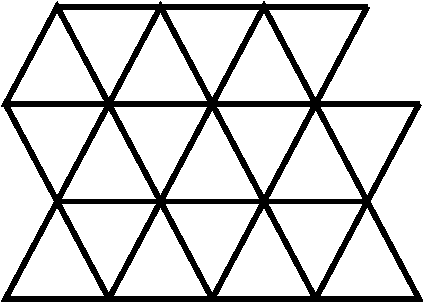
\includegraphics[height=3cm,width=4cm]{SP-11}
	\end{figure}
	If the probabilities of moving to any of the nearest neighbour sites are equal, what is the probability that the walker returns to the starting position at the end of exactly three steps?
	{	\exyear{NET/JRF(DEC-2016)}}
	\begin{tasks}(2)
		\task[\textbf{a.}]$\frac{1}{36}$
		\task[\textbf{b.}]$\frac{1}{216}$
		\task[\textbf{c.}] $\frac{1}{18}$
		\task[\textbf{d.}] $\frac{1}{12}$
	\end{tasks}
	\begin{answer}
		Solution: For walker to return to starting position it must move along an equivalent triangle in three steps.\\
		For steps one any movement can result in equilateral triangle.\\
		For step two, two out of six options will form equilateral triangle.\\
		For step three, only one out of six options will form equilateral\\ triangle Total probability $=\frac{6}{6} \times \frac{2}{6} \times \frac{1}{6}=\frac{1}{18}$\\
		So the correct answer is \textbf{Option (c)}
	\end{answer}
	\item 	An atom has a non-degenerate ground-state and a doubly-degenerate excited state. The energy difference between the two states is $\varepsilon$. The specific heat at very low temperatures $(\beta \varepsilon \gg 1)$ is given by
	{	\exyear{NET/JRF(DEC-2016)}}
	\begin{tasks}(2)
		\task[\textbf{a.}]$k_{B}(\beta \varepsilon)$
		\task[\textbf{b.}]$k_{B} e^{-\beta \varepsilon}$
		\task[\textbf{c.}] $2 k_{B}(\beta \varepsilon)^{2} e^{-\beta \varepsilon}$
		\task[\textbf{d.}]  $k_{B}$
	\end{tasks}
	\begin{answer}
		\begin{align*}
		\intertext{Assume energy at ground state is 0 and energy at first excited state is $\in$. The partition function is $Z=1+2 e^{-\beta \epsilon}$}
		\text{	Energy }&=\frac{2 \in e^{-\beta \epsilon}}{\left(1+2 e^{-\beta \epsilon}\right)}\\
		\text{Specific heat, }C_{V}&=\left(\frac{\partial U}{\partial T}\right)_{V}=\frac{2 \in e^{-\frac{\epsilon}{k T}}(-\in) \frac{-1}{k T^{2}}}{\left(1+2 e^{\frac{-\epsilon}{k T}}\right)}+\frac{2 \in e^{\frac{-\epsilon}{k T}} \in \in \frac{2}{k T^{2}}}{\left(1+2 e^{\frac{-\epsilon}{k T}}\right)^{2}}\\
		&=2 k\left(\frac{\epsilon}{k T}\right)^{2} e^{\frac{-\epsilon}{k T}} \frac{\left(1+2 e^{\frac{-\epsilon}{k T}}\right)}{\left(1+2 e^{\frac{-\epsilon}{k T}}\right)^{2}}=2 k(\beta \in)^{2} e^{-\beta \in} \frac{\left(1+2 e^{-\beta \epsilon}\right)}{\left(1+2 e^{-\beta \epsilon}\right)^{2}}\\
		C_{V} &\simeq 2 k(\beta \in)^{2} e^{-\beta \epsilon}, \quad \beta \in \rightarrow \infty
		\end{align*}
		So the correct answer is \textbf{Option (c)}
	\end{answer}
	\item In a thermodynamic system in equilibrium, each molecule can exist in three possible states with probabilities $1 / 2,1 / 3$ and $1 / 6$ respectively. The entropy per molecule is
	{	\exyear{NET/JRF(JUNE-2017)}}
	\begin{tasks}(2)
		\task[\textbf{a.}] $k_{B} \ln 3$
		\task[\textbf{b.}]$\frac{1}{2} k_{B} \ln 2+\frac{2}{3} k_{B} \ln 3$
		\task[\textbf{c.}]$\frac{2}{3} k_{B} \ln 2+\frac{1}{2} k_{B} \ln 3$
		\task[\textbf{d.}] $\frac{1}{2} k_{B} \ln 2+\frac{1}{6} k_{B} \ln 3$
	\end{tasks}
	\begin{answer}
		\begin{align*}
		S&=-k_{B} \sum_{i} P i \ln P i\\
		P_{1}&=\frac{1}{2}, P_{2}=1 / 3 \text { and } P_{3}=1 / 6 \\
		S&=-k_{B}\left(\frac{1}{2} \ln 1 / 2+1 / 3 \ln 1 / 3+1 / 6 \ln 1 / 6\right) . \\
		&=-k_{b}\left(\frac{1}{2}(\ln 1-\ln 2)+\frac{1}{3}(\ln 1-\ln 3)+\frac{1}{6}(\ln 1-\ln 6)\right. \\
		&=k_{B}\left[\frac{1}{2} \ln 2+\frac{1}{3} \ln 3+\frac{1}{6} \ln 2+\frac{1}{6} \ln 3\right]=k_{B}\left[\frac{1}{2} \ln 2+\frac{1}{6} \ln 2+\frac{1}{3} \ln 3+\frac{1}{6} \ln 3\right] \\
		S&=k_{B}\left[\frac{3 \ln 2+\ln 2}{6}+\frac{2 \ln 3+\ln 3}{6}\right]=k_{B}\left(\frac{4 \ln 2}{6}+\frac{3 \ln 3}{6}\right)=k_{B}\left[\frac{2}{3} \ln 2+\frac{1}{2} \ln 3\right]
		\end{align*}
		So the correct answer is \textbf{Option (c)}
	\end{answer}
\end{enumerate}